\documentclass{article}
\usepackage[utf8]{inputenc}

\usepackage{amsmath,amsthm, amssymb}
\usepackage{mathrsfs}
% \usepackage[margin=3.0cm]{geometry}
\usepackage{mathtools}
\usepackage{dsfont}
\usepackage{xcolor}
\usepackage{xfrac}
\usepackage{algorithm,algpseudocode}
\usepackage{todonotes}
\usepackage{qcircuit}
\usepackage{smartref}
\usepackage{graphicx}
\usepackage{tikz}
\usetikzlibrary{topaths,calc}



%%%%%%%%    NOTATION DEFINITIONS FOR EASIER WRITING
\newcommand{\ket}[1]{|#1\rangle}
\newcommand{\bra}[1]{\langle #1|}
\newcommand{\braket}[2]{\langle #1|#2\rangle}
\newcommand{\ketbra}[2]{| #1\rangle\! \langle #2|}
\newcommand{\parens}[1]{\left( #1 \right)}
\newcommand{\brackets}[1]{\left[ #1 \right]}
\newcommand{\abs}[1]{\left| #1 \right|}
\newcommand{\norm}[1]{\left| \left| #1 \right| \right|}
\newcommand{\diamondnorm}[1]{\left| \left| #1 \right| \right|_\diamond}
\newcommand{\anglebrackets}[1]{\left< #1 \right>}
\newcommand{\set}[1]{\left\{ #1 \right\}}
\newcommand{\ceil}[1]{\left\lceil #1 \right\rceil}
\newcommand{\openone}{\mathds{1}}
\newcommand{\expect}[1]{\mathbb{E}\brackets{#1}}
\newcommand{\prob}[1]{\text{Pr}\left[ #1 \right]}
\newcommand{\textprob}[1]{\text{Pr}\left[ \text{#1} \right]}
\newcommand{\bigo}[1]{\mathcal{O}\left( #1 \right)}
\newcommand{\bigotilde}[1]{\widetilde{\mathcal{O}} \left( #1 \right)}
\newcommand{\ts}{\textsuperscript}
\newcommand{\field}{\mathbb{C}}


%%%%%%%%    VARIABLE DEFINITIONS FOR EASY CHANGING LATER
\newcommand{\calX}{\mathcal{X}}
\newcommand{\calY}{\mathcal{Y}}
\newcommand{\calZ}{\mathcal{Z}}


%%%%%%%%    OPERATOR DEFINITIONS FOR EASIER MATHS
\DeclareMathOperator{\Tr}{Tr}
\DeclareMathOperator{\Hom}{Hom}
\DeclareMathOperator{\card}{card}
\DeclareMathOperator{\cspan}{span}
\newcommand{\cardi}[1]{\card \parens{ #1 }}
\newcommand{\trace}[1]{\Tr \brackets{ #1 }}
\newcommand{\partrace}[2]{\Tr_{#1} \parens{ #2 }}

\newcommand{\complex}{\mathbb{C}}
\newcommand{\matn}{\mathbb{M}_n}
% \newcommand{\identity}{\mathbbm{1}}
\newcommand{\identity}{\mathds{1}}
\newcommand{\ident}{\mathbb{I}}
\newcommand{\hilbspace}{\mathscr{H}}
\newcommand{\partfun}{\mathcal{Z}}
\newcommand{\si}{\vec{s}_i}
\newcommand{\fullProj}{\widetilde{\Pi}}
\newcommand{\basei}{\ket{s_i}}
\newcommand{\base}[1]{\ket{s_{#1}}}
\newcommand{\duali}{\bra{s_i}}
\newcommand{\dual}[1]{\bra{s_{#1}}}

\newtheorem{theorem}{Theorem}
\newtheorem{lemma}[theorem]{Lemma}
\newtheorem{claim}[theorem]{Claim}
\newtheorem{corollary}[theorem]{Corollary}
\newtheorem{defn}{Definition}
% \DeclareMathOperator*{\dim}{dim}

\newcommand\disjointUnion{\rotatebox[origin=c]{180}{$\prod$}}

\title{Properties of Random and Quantum Walks on Hypergraphs}
\author{Matthew Hagan}
\date{\today}

\begin{document}



\maketitle
\begin{abstract}
	We study hypergraphs as linear operators acting on a vector space constructed from the power set of an underlying node set. We first show a simple construction of this vector space, which we call the hyperspace, and highlight convenient operators. We then study linear operators on this hyperspace and show how it leads to a linear theory of directed, weighted hypergraphs. To highlight the utility of this construction we investigate the differences between the complete hypergraph of $n$ nodes and the complete graph on $2^n$ nodes.
\end{abstract}
% \tableofcontents

\section{Introduction}
Graph theory has become a ubiquitous facet of computational and network sciences. The utility of graphs in quantitative sciences is hard to understate, as it has proven incredibly convenient to study pairwise interactions between elements of some model. This notion has been generalized to objects known as hypergraphs, which attempt to allow for interactions between more than two elements. Although this theoretically allows for much richer models, studying hypergraphs mathematically has proven difficult as there are many ambiguities in what quantities are important to consider. Nevertheless, hypergraphs have been used as compact models in diverse areas such as machine learning recommender systems \cite{hgRecSystems}, databases \cite{databases}, bioinformatics \cite{bioinformatics}, Steiner Tree problems \cite{Brazil2015}, and 3CNF satisfiability formulas \cite{3cnf}.

Before developing our own proposal for a useful hypergraph quantity or framework \cite{xkcd} we first provide a brief survey of recent hypergraph literature. Some common concepts explored in existing hypergraph literature are notions of clustering, cuts, random walks, and singular values of tensors.
Several notions for clustering have been explored, one particularly recent development has been the notion of ``$s$-distance" developed Sinan et. al \cite{sinanPNNL}. In \cite{sinanPNNL}, they develop a notion of a constrained walk on undirected hypergraphs, where the paramater $s$ dictates the minimum intersection required between edges to be traversable. Exploring this constrained walk they develop metrics that relate how connected vertices or groups of vertices are via $s$. Cuts on hypergraphs have been studied extensively, one of the earlier papers establishing the area by Lawler \cite{lawler_cutsets_1973}. Further extensions to the simple concept of a cut has been explored extensively, see \cite{veldt_hypergraph_2020}, \cite{rafaellaCheeger}, \cite{ageev_approximation_nodate}, and \cite{conlon_hypergraph_2019} for various developments. Random walks and spectral theories for hypergraphs have been developed mostly as a coupled concept. This area gets fairly technical quickly, see \cite{rough_spectral_tensors}, \cite{sinan_random_walks_laplacians_clustering}, \cite{jost_hypergraph_2018}, or \cite{mulas_random_2021} for possible entry points to further literature.

The main focus of this paper is to explore the structure of the vector space in which hypergraphs act on and to define somewhat natural quantities related to this space. We will introduce some useful notation and theorems in Section \ref{sec:preliminaries}. In Section \ref{sec:hyperspace} we will develop this space, which we call the hyperspace, in a rigorous manner. We will follow this definition up by describing some useful matrices and exploring how previous definitions fit in the hyperspace language. In Section \ref{sec:cardinality} we extend the notion of set cardinality to apply to vectors in an associated hyperspace. We show that this is a useful quantity to consider when studying hypergraph dynamics and use cardinality to distinguish between a complete hypergraph and a complete graph acting on the same size vector space. We then introduce a quantity we call the average cardinality of a hypergraph.
In Section \ref{sec:algorithms} we introduce classical and quantum algorithms for computing this average cardinality. We also posit a few decision problems and leave their computational complexity for future work.



% Before diving into our constructions, we first would like to provide a small, shallow survey of the field of hypergraph network sciences. The paper by Gallo et. al. \cite{gallo1993directed}

% Before a spectral theory of hypergraphs can be defined, a decent notion of spectral graph theory is good to have in mind. A graph $G$ is typically viewed as two sets $G = (N, E)$, one set $N = \set{n_i}_{i=1}^n$ of nodes ($V$ is reserved for vector spaces later) and one set of edges $E = \set{(n_a, n_b, w_{a,b})}$, where $n_a$ represents the head node and $n_b$ the tail, if this edge is directed, and $w_{a,b} \in \field$ the weight. The field $\field$ is left arbitrary for now, all we require is that the edge weights be in a field so we can construct vector spaces later.


% maybe talk about applications of spectral graph theory?

\section{Preliminaries} \label{sec:preliminaries}
We will use $N$ to denote a set of nodes, typically $N = \set{n_i}_{i=1}^n$, as opposed to using the more common $V$ for vertices as we will use $V$ to denote vector spaces later on. The power set $2^N$ can be decomposed into a direct sum of families of sets based on their cardinality. For a cardinality $k$ let  $N_k \coloneqq \set{X \subseteq N : |X| = k}$, which gives the decomposition $2^N = \bigcup_{k=0}^n N_k$. Note that we will also use the symbol $\bigoplus$ to denote the disjoint union, as this notation will match with the direct sum for vector spaces, which gives $2^N = \bigoplus_{k=0}^n N_k$. 

We will rely heavily on the use of free modules to construct vector spaces. Although free modules are defined for general rings, we will restrict our attention to $\field$ so that we can think of these modules as vector spaces. Intuitively, the free module of a set assigns a group element to each member of the set; in other words each element of the set is assigned a basis vector and the vector space is then the linear span of all the basis vectors. The use of the field $\field$ is a crutch that should be easily removed in subsequent work if need be. We will rely on Dirac notation $\ket{x}$ to denote vectors, note that we explicitly do \emph{not} require kets to be unit normalized. 

As a small example we will work out the free module of the set $X = \set{x_1, x_2}$. We will denote the free module of the set $X$ as $\mathcal{F}(X)$, which gives two basis vectors $\ket{x_1}$ and $\ket{x_2}$. We can say that the span of these vectors is roughly equal to the free module, $\cspan (\ket{x_1}, \ket{x_2}) = \mathcal{F}(X)$. As this is somewhat of a homework problem, we will state but not prove the following claim.
\begin{claim}
\begin{equation}
\mathcal{F}(A \bigoplus B) = \mathcal{F}(A) \bigoplus \mathcal{F}(B)    
\end{equation}
\end{claim}
This is rather intuitive, if we take the disjoint union of two sets and give each element a basis vector this is the same as giving a basis vector to each set separately and taking the direct sum of the two spaces.

\section{Hypergraph Construction} \label{sec:hyperspace}

Hypergraphs are a direct generalization of a graph, as such it will be useful to review the construction of graphs in a similar framework that we will develop hypergraphs. A graph $G$ is defined as a tuple of sets $G = (N, E)$, where $N$ represents the set of nodes $N = \set{n_i}_{i=1}^n$ and $E$ the set of edges. We will work with directed and weighted edges denoted as $e = (n_a, n_b, w_{a,b})$. For this edge between node $n_a$ and $n_b$ with weight $w_{a,b}$ we will denote the input node as $\alpha(e) \coloneqq n_a$ and the output node $\beta(e) \coloneqq n_b$, with the weight of the edge either denoted by a subscript or the simple $w(e)$. Note that when the underlying graph is implied we use $w_{a,b}$ to denote the edge weight from $a$ to $b$, with the weight 0 if no such edges exist.

We now construct the vector space that graphs act on. Let $V_G = \mathcal{F}(N)$ denote the vector space with basis $\ket{n_i}$ for $i = 1$ to $n$. The matrix of primary importance is the adjacency matrix, which is typically defined with entries taking values 0 or 1 but we will allow it to take elements in $\field$ for convenience. The adjacency matrix $A_G$ has the entry $(i,j)$ defined as the total edge weight going \emph{from} node $j$ \emph{to} node $i$. This may seem backwards, but this allows us to use inner products in a convenient fashion: $w_{i,j} = \bra{j} A_G \ket{i}$. This backward-ness stems from the author's preference of using column vectors over row vectors. 

We briefly define three other helpful matrices, starting first with the degree matrix. The degree matrix $D_G$ is most easily defined in terms of the degree function $\deg (i) \coloneqq \sum_{k = 1}^n | w_{i, k}|$ which intuitively tells you the amount of "weight" leaving a node as a positive real number. From this we define the degree matrix as $[D_G]_{i,j} \coloneqq \delta_{i,j} \deg (i)$, where the $G$ may be dropped if the graph is implied. 

The second matrix is the classical walk operator $W_{G}$, which is essentially an $L_1$ normalized adjacency matrix
\begin{equation}
[W_G]_{i,j} \coloneqq 
    \begin{cases}
        \frac{|[A_G]_{i,j}|}{\deg (j)} & \text{ if } \deg (j) > 0 \\
        \delta_{i,j} & \text{ if } \deg (j) = 0.
    \end{cases}
\end{equation}
In other words, we shift all edge weights to be between 0 and 1 and normalize via the degree. If a node has no outgoing edges we simply add a loop for a walker to stay put. This matrix $W_G$ is stochastic and maps probability vectors to probability vectors. If we were to define an $L_2$ normalized walk matrix, which is useful for quantum mechanics, then we would keep the edge weights as complex values and normalize by $\sum_{k} | w_{i,k} |^2$ as opposed to the degree. For concreteness, we will use the letter $U_G$ to denote the $L_2$ normalized walk matrix, which is unitary as opposed to stochastic. Similarly, if a node has no outgoing weight we simply add a weight 1 self-loop to the walk operator.

The final matrix is the non-normalized Laplacian, $L_G \coloneqq D_G - A_G$. This matrix, along with the adjacency and walk matrices to a slightly lesser degree, constitutes the primary object of study for spectral graph theory. In spectral graph theory typically only unweighted, undirected graphs are considered. We can define the normalized Laplacian $\mathcal{L}_G \coloneqq D_G^{+1/2} L_G D_G^{+1/2} = \identity - D_G^{+1/2} A_G D_G^{+1/2}$, where $+1/2$ denotes the square root of the Moore-Penrose pseudoinverse. When normalization is unspecified "Laplacian" will typically refer to the normalized variant. The non-normalized Laplacian $L_G$ can be made column or row stochastic by multiplying $L_G$ by $D_G^{+}$ on the right or left respectively (or vice-versa).

We now shift our attention to hypergraphs. A hypergraph $H$ is defined as a tuple $H = (N, E)$, where $E$ now constitutes a set of hyperedges. We will specify if a given $E$ refers to hyperedges or graph edges if the context is unclear. A hyperedge $e \in E$ maps a subset $A \subseteq N$ to another subset $B \subseteq N$ with weight $w_{A, B}$. Note we explicitly allow for the empty set $\varnothing = \set{}$. This is a directed and weighted hyperedge and is denoted $e = (A, B, w_{A,B})$. As with graphs we will use the functions $\alpha$ to denote the input subset, $\beta$ the output subset, and $w$ the weight. Note that the most commonly studied hypergraphs in the literature consist of ``undirected" and unweighted hyperedges, where an ``undirected" edge simply refers to a subset $A \subseteq N$. We note that this notion of ``undirected" will prove cumbersome later, so we prefer to use an undirected edge as one which maps $A \to B$ and $B \to A$, not as a single subset. If necessary, we will refer to the previously defined ``undirected" edges as "blob" type edges as they are typically drawn as blobs of nodes.



To study linear operators related to hypergraphs we will need to construct a slightly more intricate vector space. To start, we note the following useful property of the power set 
\begin{equation}
    2^N =  \bigcup_{k=0}^{|N|} N_k = \bigoplus_{k=0}^{k = |N|} N_k,
\end{equation}
where $N_k := \set{X \subseteq N : |X| = k}$ is the set of subsets of $N$ of cardinality $k$ and we use $\bigoplus$ to denote the disjoint union, or coproduct, when working in the category Set. We will use $s_i$ to denote a single arbitrarily indexed subset of $N$, so $2^N = \set{s_i}_{i=1}^{2^n}$. Given this, we now introduce the main vector space of this paper.

\begin{defn}[Hyperspace]
    Let $F$ denote the free module action and $N = \set{n_i}_{i=1}^n$. We call the vector space $$V \coloneqq F \parens{2^N} = F \parens{\bigoplus_{k=0}^n N_k} = \bigoplus_{k=0}^n F(N_k) = \bigoplus_{k=0}^n V_k $$ associated with a hypergraph the hyperspace. A hyperspace $V$ comes with projectors $\Pi_k : V \to V_k$ and inclusions $\iota_k : V_k \to V$. We denote the useful combination $\fullProj_k \coloneqq \iota_k \circ \Pi_k : V \to V$ which acts as
    \begin{equation}
        \fullProj_k \basei = \begin{cases}
            0 & \text{if } s_i \notin N_k \\
            \basei & \text{if } s_i \in N_k .
        \end{cases}
    \end{equation} We denote the seemingly natural basis $\basei$, where each $s_i \subseteq N$ is an indexed subset of $N$ the subset basis of the hyperspace.
\end{defn}

We now can define the adjacency matrix for the hypergraph
\begin{equation}
    A_H \coloneqq \sum_{e \in E} w(e) \ketbra{\beta(e)}{\alpha(e)},
\end{equation}
where each edge simply maps the vector associated to the input set $\alpha(e)$ to the vector associated with it's output set $\beta(e)$ with weight $w(e)$. From this matrix we can compute the $L_1$ out-degree of a subset as
\begin{equation}
    \deg(s_i) \coloneqq \sum_{s_j \in 2^N} \abs{\dual{j} A_H \basei}
\end{equation}

This matrix allows us to define the $L_1$ degree matrix
\begin{equation}
    D_H \coloneqq \sum_{s_i \in 2^N} \deg(s_i) \ketbra{s_i}{s_i}.
\end{equation}
Note if a hypergraph has no edges with a given subset as it's input then it's out-degree is 0. One could also characterize an in-degree but we will not have use for such a quantity.

The $L_1$ out degree now allows us to define a random walk process on any given hypergraph. Define the walk operator $W_H$ as follows
\begin{equation}
    \dual{i} W_H \base{j} \coloneqq \begin{cases}
        \frac{\abs{\dual{i} A_H \base{j}}}{\dual{j} D_H \base{j}} & \deg(s_j) > 0 \\
        \delta_{i,j} & \deg(s_j) = 0.
    \end{cases}
\end{equation}
We briefly show that this is a stochastic matrix, starting with subsets $s_i$ that have non-zero out-degree:
\begin{align}
    \deg(s_j) > 0 \implies \sum_{s_i \in 2^N} \dual{i} W_H \base{j} &= \sum_{s_i \in 2^N } \frac{\dual{i} A_H \base{j}}{\dual{j} D_H \base{j}} \\
    &= \frac{1}{\deg(s_j)} \sum_{s_i} \abs{\dual{i} A_H \base{j}} \\
    &= 1.
\end{align}
The case where $\deg(s_j) = 0$ is trivial. Note that this can be expressed as $W_H = A_H D_H^{+}$, where we remind the reader $M^+$ denotes the pseudo-inverse.

We now investigate quantum walks over a given hypergraph. Unfortunately the situation is not as straightforward as the random walk case, where we can simply reweight all outgoing edges from a subset by that subset's out-degree. This can't be replicated for quantum walks as the unitary matrix must be of full rank, which is not guaranteed for any arbitrary adjacency matrix of a hypergraph. Moreover, the procedure of adding self-loops to subsets that do not have outgoing edges does not solve the rank issue.

For quantum walks we have to add a node and expand our vector space. We construct the Hermitian matrix $\widetilde{A}_H \coloneqq A \otimes \base{0}\dual{0} + A^* \otimes \base{1} \dual{1}$. Then to construct the unitary we take $U_H = e^{i\widetilde{A}_H}$. Unfortunately this construction essentially makes the adjacency matrix ``non-local'', as it takes the sum of all possible powers of the adjacency matrix which spreads a walker from a single subset over all possible subsets it could be connected to. This process is rather cumbersome so we will instead study unitary adjacency matrices, denoted $U_H$ as opposed to constructed unitary matrices from given hypergraphs.

The last matrix to consider for hypergraphs is the Laplacian $L_H$. We will simply port the definitions from graphs over
\begin{equation}
    L_H \coloneqq D_H - A_H, \quad \mathcal{L}_H \coloneqq D_H^{+1/2} L_H D_H^{+1/2}.
\end{equation}
We make note of a few properties of this matrix:
\begin{itemize}
    \item PSD?
    \item Stochastic?
    \item Diff Eq solution?
    \item IDK?
\end{itemize}
Once these properties are filled in then this section should be good to go I think.

\begin{figure}
    \centering
    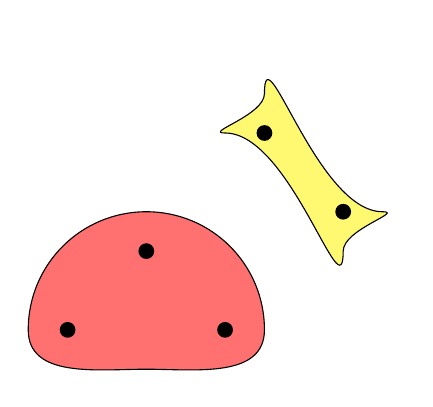
\begin{tikzpicture}
        \node (n1) at (0,0) {};
        \node (n2) at (1,1) {};
        \node (n3) at (2,0) {};
        \node (n4) at (2.5, 2.5) {};
        \node (n5) at (3.5, 1.5) {};
        \node (e1) at (1,0.5) {};
        \node (e2) at (3, 2) {};

        \begin{scope}[fill opacity=0.8]
            \filldraw[fill=red!70] ($(n1)+(-0.5,0)$) 
                to[out=90,in=180] ($(n2) + (0,0.5)$) 
                to[out=0,in=90] ($(n3) + (0.5,0)$)
                to[out=270, in=0] (1, -0.5)
                to[out=180, in=270] ($(n1) + (-0.5, 0)$);
            \filldraw[fill=yellow!70]
            ($(n4) + (0, 0.5)$)
            to[in=180, out=90] ($(n5) + (0.5, 0)$)
            to[in=90, out=0] ($(n5) + (0, -0.5)$)
            to[in=0, out=270] ($(n4) + (-0.5, 0)$)
            to[in=270, out=180] ($(n4) + (0, 0.5)$);
        \end{scope}

        \foreach \v in {1,2,3,4,5} {
            \fill (n\v) circle (0.1);
        }
        % [line width=1pt, double distance=3pt,
        %      arrows = {-Latex[length=0pt 3 0]}] $(e1)$ -- $(e2)$;
    \end{tikzpicture}
    \caption[Hypergraph]{An example of a directed, weighted hypergraph with a single edge $e$}
\end{figure}



\section{Cardinality} \label{sec:cardinality}
We now introduce the main quantity relevant for our study of hypergraphs action on vectors, what we have termed ``cardinality''. We will define a random variable $\card$ for a given vector in hyperspace and show different ways to extract this quantity from a given hypergraph. Then we will define a cardinality matrix $C$ from a given hypergraph and define the cardinality scrambling for a hypergraph. 

\subsection{Vector Cardinality}
\begin{defn}[Vector Cardinality]
    Define the random variable $\cardi{\ket{\psi}}$, which is supported over the set $\set{0, 1, 2, \ldots, n}$ to have the following distribution:
    \begin{equation}
        \prob{\cardi{\ket{\psi}} = k} \coloneqq \frac{\sum_{i} \abs{\dual{i} \fullProj_k \ket{\psi} }}{\sum_j \abs{\braket{s_j}{\psi}}}.
    \end{equation}
\end{defn}
Is this a distribution? I think so
\begin{align}
    \sum_i |\dual{i} \fullProj_k \ket{\psi} | &= \sum_{s_i \in N_k} \abs{\braket{s_i}{\psi}}.
\end{align}
We then have
\begin{equation}
    \sum_j \abs{\braket{s_j}{\psi}} = \sum_{k=0}^n \sum_{s_i \in N_k} \abs{\braket{s_i}{\psi}}.
\end{equation}
Therefore
\begin{align}
    \sum_{k=0}^n \prob{\cardi{\ket{\psi}} = k} &= \sum_{k=0}^n \frac{\sum_{i} \abs{\dual{i} \fullProj_k \ket{\psi} }}{\sum_j \abs{\braket{s_j}{\psi}}} \\
    &= \frac{\sum_{k=0}^n \sum_{s_i \in N_k} \abs{\braket{s_i}{\psi}} }{\sum_{k=0}^n \sum_{s_i \in N_k} \abs{\braket{s_i}{\psi}}} \\
    &= 1.
\end{align}
Given the presence of $\ket{\psi}$ in the denominator $\frac{1}{\sum_i \abs{\braket{s_i}{\psi}}}$ in the definition of $\card$ we note that this quantity is not defined for the zero vector. 

Given a vector $\ket{\psi}$ one could also define a cardinality quantum state by keeping phases coherent upon collapse to cardinality $k$. This would look like
\begin{equation}
    \card_Q\parens{\ket{\psi}} = \sum_{k=0}^n \frac{\sum_{s_i \in 2^N} \dual{i} \fullProj_k \ket{\psi}  }{\sqrt{\sum_{s_j \in 2^N} \abs{\braket{s_j}{\psi}}^2}} \ket{k}
\end{equation}

Now that we have a cardinality distribution for a given vector, we can now study the interaction of cardinality with hypergraphs.
\begin{defn}[Average Cardinality]
    Given a hypergraph $H$, let $W_H$ denote the unique column stochastic walk operator. As $W_H \ket{\psi}$ will never be a zero vector we can define the random variable
    \begin{equation}
        \gamma(H) \coloneqq \int \cardi{W_H \ket{\psi}} d\ket{\psi}.
    \end{equation}
\end{defn}
From this definition we can also define the dominant cardinality for aperiodic, irreducible random walks:
\begin{defn}[Dominant Cardinality]
    Given a stochastic operator $W_H$ that is aperiodic, non-bipartite, and irreducible then $W_H$ satisfies the Peron-Frobenius theorem and has a unique dominant eigenvector with eigenvalue 1. This allows us to define the random variable
    \begin{equation}
        \Delta(W_H) \coloneqq \lim_{k \to \infty} \gamma(W_H^k).
    \end{equation}
\end{defn}

\subsection{Cardinality Matrix}
We now pivot to an alternative way to studying how a given hypergraph $H$ affects the cardinality of states in it's hyperspace. Our aim is to do so by studying properties of the matrix as opposed to it's action on all vectors over the hyperspace. Our goal is to show when these two notions offer equivalent insights into a hypergraphs behavior.

\begin{defn}[Cardinality Matrix]
    Given a hypergraph $H$ with adjacency matrix $A_H$, define the $(n+1) \times (n+1)$ matrix $C_H$ as
    \begin{equation}
        \bra{i} C_H \ket{j} \coloneqq \sum_{s_i \in N_i} \sum_{s_j \in N_j} \dual{i} A_H \base{j}.
    \end{equation}
\end{defn}
Intuitively $C_H$ captures the edge weight in $H$ that transfers vectors of cardinality $j$ to cardinality $i$. 




\subsection{Complete Graph vs. Complete Hypergraph}
We now look at the complete graph $G_C$ over $2^N$ and compare it against the complete hypergraph $H_C$ over $N$. Let $\ket{e} = \frac{1}{\sqrt{2^n}} \sum_{i=1}^{2^n} \ket{s_i}$ denote the $L_2$ normalized all ones vector in the subset basis. The walk operator, or adjacency operator, for the complete hypergraph is then simply $H_C = \ketbra{e}{e}$, or the all ones matrix properly normalized. As a hypergraph we have access to the $\card$ operator, which allows us to compute the cardinality distribution of the dominant eigenvector of $H_C$ as
\begin{align}
    \cardi{H_C(n), k} := \prob{\cardi{\ket{e}} = k } = \frac{\binom{n}{k}}{2^n}.
\end{align}
We can generalize this notion to an arbitrary stochastic hypergraph $H$  by replacing $\ket{e} \mapsto \lim_{m \to \infty} \int H^m \ket{\psi} ~d\ket{\psi} $, which is simply a method of obtaining the dominant eigenvectors.


\begin{align}
    \binom{n}{k} &= \frac{n!}{(n-k)! k!} \\
    &= \frac{(1 + o(1))\sqrt{2 \pi n} n^n e^{-n}}{(1+o(1)) 2 \pi \sqrt{n (n-k)} k^k (n-k)^{n-k} e^{-n}} \\
    &= \frac{1 + o(1)}{\sqrt{2 \pi}(1+o(1))} \frac{n^n}{ k^k (n-k)^{n-k + 1/2}}
\end{align}

For the complete hypergraph we note that we can easily compute quantities such as the expected cardinality and the entropy
\begin{align}
    \expect{\cardi{H, k}} &= \frac{n}{2} \\
    \mathbf{H} \brackets{\cardi{H, k}} &= - \sum_{k=0}^{n} \frac{\binom{n}{k}}{2^n} \log \parens{\frac{\binom{n}{k}}{2^n}}\\
\end{align}

\section{Algorithms} \label{sec:algorithms}

\section{Algebraic Construction}
Now that we have a vector space, we can define a hyperedge $e$ simply as a linear map on this overall vector space, or in other words as a $\field$-module endomorphism
\begin{equation}
    e \in \Hom_{\field} (V, V).
\end{equation}
This condition of linearity is per usual. We say $e$ is a $\field$-module homomorphism (aka linear map) if for all scalars $c \in \field$ and vectors $u, v \in V$
\begin{align}
    e(c * v) = c * e(v) \\
    e (u + v) = e(u) + e(v).
\end{align}
Note that we can add elements of $V$ due to the underlying abelian group structure of the module. 

We then take another step and ask the question, can we induce a module structure on the set of linear maps $\Hom_{\field}$? Since $\field$ is a field we are allowed to do so (we only really need commutativity of $\field$ ). First define the action of $c \in \field$ on $e \in \Hom_\field(V, V)$ in the obvious way $(c * e) (v) := c * e(v)$. This may seem like simply removing the parenthesis, but the question of linearity shows it is a different matter:
\begin{align}
    (c * e) (s * v) &= c * e( s * v) \\
    &= (c * s) * e(v) \\
    &\overset{!}{=} s * (c * e) (v),
\end{align}
where the ! means we used commutativity to get $(c *e) (s * v) = s * (c * e) (v)$. Addition follows straightforwardly, $(e+f) (v) \coloneqq e(v) + f(v)$. This all may seem redundant, but it's important to spell out that everything is legal.

So we now have hyperedges defined as a specific linear map $e$ acting on a vector space $V$, and that we can add hyperedges and multiply them by some field. We then can simply define a hypergraph $h = \sum c_i e_i$, a weighted sum of hyperedges. Thats it! 


\section{Scratch}

\begin{theorem}[Stirling's]
    \begin{equation}
        n! = (1 + o(1)) \sqrt{2 \pi n} n^n e^{-n}
    \end{equation}
    \begin{proof}
    \begin{align}
        n! &= \int_0^\infty t^n e^{-t} dt \\
        &= \int_0^\infty (s+n)^{n} e^{-(s+n)} ds \\
        &= n^n e^{-n} \int_0^\infty \parens{ 1 + \frac{s}{n}}^{n} e^{-s)} ds \\
        &= n^n e^{-n + n \log n} \int_0^\infty e^{n \log \parens{1 + \frac{s}{n}} - s} ds \\
        &= n^n e^{-n + n \log n} \int_0^\infty e^{n \log \parens{1 + \frac{s}{n}} - s} ds \\
        &= \int_0^\infty t^n e^{-t} dt 
    \end{align}
\end{proof}
\end{theorem}

A linear theory of hypergraph connections allows for immediate generalizations of many previous concepts. We posit a few conjectured areas that could lead to fruitful future research.
\begin{itemize}
    \item There is a beautiful theorem by Sunada that states that a graph $G$ is an optimal expander, aka the graph is Ramanujan, if and only if it's Ihara zeta function satisfies a Graph variant of the Riemann Hypothesis. Our theory now allows for these questions to be generalized to the hypergraph setting.
    \item One can impose that a hypergraph maintains the global vector given a certain norm, for example an $L_1$ normalized theory would consitute a model that conserves probability. If one defines a parametrization of the probability of each of these edges how does an observed data point update these models? Algorithms that could efficiently perform updates of all models seems unlikely, but what constrictions could lead to efficient bayesian updates?
    \item Previous definitions of hypergraphs have noted a duality between nodes and edges, as in there is a one-to-one mapping between a graph with edge sets and vertex sets swapped in a well defined manner. How does this duality affect the spectral properties of the hypergraph connections?
    \item Neural Networks are constructed by creating a set of nodes, assigning each a number, and then imposing a directed graph structure with weighted edges from each layer to the next. This theory allows for a linear version of a neural network that connects multiple nodes in one layer to multiple nodes in the next while retaining single node connections.
    \item A common thread in modern algorithms is the ability to compute global properties of an object from local information. For example the PCP theorem states that a computational proof can be verified with high probability by only accessing a constant number of bits from the proof. Conceptually a global property of a string of bits can be verified through only local information. How can one define local and global properties on hypergraphs?
    \item  A current area of study known as Topological Data Analysis (TDA) attempts to study topological properties of an underlying manifold $X$ via a collection of 0 dimensional samples (aka points in $\mathbb{R}^n$). These points are then used to construct a graph via the usual Euclidean metric on
    \item Graphs induce a unique linear hypergraph via the action of powering. For example specifically look at edges in the space $V_2$.  
\end{itemize}

\section*{Acknowledgements}

\bibliographystyle{unsrt}
\bibliography{bib}


\end{document}
